%%%%%%%%%%%%%%%%%%%%%%%%%%%%%%%%%%%%%%%%%%%%%%%%
%%%%%%%%%%%%%Przykładowy dokument%%%%%%%%%%%%%%%
%%%%%%%%%%Wraz z klasą pracadyp.cls%%%%%%%%%%%%%
%%daje w ShareLatex w pełni czytleny plik .pdf%%
%%%%dla Otwartego Systemu Antyplagiatowego%%%%%% 
%%%%%%%WMP.SNŚ UKSW, Marek A. Kowalski%%%%%%%%%%
%%%%%%%%%%%%%%%%%%%%%%%%%%%%%%%%%%%%%%%%%%%%%%%%
\documentclass[licencjacka]{pracadypl}
%
%% ważne definicje %%
%\usepackage{tgtermes}
\usepackage[T1]{fontenc}
\usepackage{polski}
\usepackage[utf8]{inputenc}
\usepackage{hyperref}
\hypersetup{
	colorlinks,
	citecolor=black,
	filecolor=black,
	linkcolor=black,
	urlcolor=black
}
\input glyphtounicode
\pdfgentounicode=1
\usepackage{amssymb, amsthm,amsmath, tikz, indentfirst}
\hyphenation{for-singiem}
\bibliographystyle{plain}
%\usepackage{showkeys}
\newtheorem{tw}{Twierdzenie}[chapter]
\newtheorem{np}[tw]{Przykład}
\newtheorem{obs}[tw]{Obserwacja}
\newtheorem{fakt}[tw]{Fakt}
\newtheorem{wn}[tw]{Wniosek}
\theoremstyle{definition}
\newtheorem{de}{Definicja}

\DeclareMathOperator{\spacja}{\hspace{0,1cm}}
\newcommand{\linia}{\rule{\linewidth}{0.4mm}}

\usepackage{float}

\def\uczelnia{{Uniwersytet Kardynała Stefana Wyszyńskiego w~Warszawie}\\
	Wydział Matematyczno-Przyrodniczy \\ Szkoła Nauk Ścisłych}
\def\mgr{magisterska}
\def\lic{licencjacka}
\def\inz{inżynierska}
\def\sk{Słowa kluczowe}
\def\dz{Dziedzina Socrates-Erasmus}
\def\et{English title}
\def\kt{Klasyfikacja tematyczna}
\author{Jacek Giedronowicz}
\nralbumu{95175}
\title{Rekomendacja stron www za pomocą silnika Apache Lucene }
\kierunek{Informatyka}
\zakres{Machine Learning}
% Praca wykonana pod kierunkiem:
% (Podając w dopełniaczu tytuł stopień imię i nazwisko opiekuna pracy
% trzeba pamiętać, że w tym przypadku prawidłową formą skrótu słowa doktor 
% jest dr w odniesieniu do kobiet i dr. w odniesieniu do mężczyzn. Możemy więc
% przykładowo zapisać, że praca została wykonana pod kierunkiem 
% prof. dr hab. Ewy Rak i prof. dr. hab. Adama Raka. Pominięcie kropki po 
% drugim "dr" byłoby błędem.
\opiekun{dr. Roberta Kłopotka}
% miesiąc i rok:
\date{Lipiec 2020}
%Słowa kluczowe:
\keywords{-}
%Podać dziedzinę pracy wg klasyfikacji Socrates-Erasmus:
\dziedzina{ 
	%11.1 Matematyka
	11.3 Informatyka 
	%13.3 Chemia
	%% pełny wykaz jest w pliku 
	%% http://www.mish.uw.edu.pl/pliki/kody_erazmus.pdf
}
%Klasyfikacja tematyczna według AMS (matematyka) lub ACM (informatyka) ...
\klasyfikacja{Machine Learning}
\tytulang{Website recommendation using the Apache Lucene engine}
%% koniec ważnych definicji %%
%
%%% autorskie definicje %%%
%%% koniec autorskich definicji %%%
%

\begin{document}
\maketitle
\tableofcontents
\thispagestyle{empty}

\chapter{Wprowadzenie}

\linia
\begin{itemize}
	\item ok 1-2 str
	\item ogólne zagadnienie jak jest stosowane w praktyce (do przewidywania)
	\item opis, że klasyfikacja jest trudna, używa się wielu metod, że jednym z podejść jest komitet klasyfikatorów, aby poprawić skuteczność
	\item cel pracy, hipotez badawczych
	\item krótki opis co jest w danym rozdziale
\end{itemize}
	

\linia

\chapter{Stan rynku}

\linia
\begin{itemize}
	\item przede wszystkim zdefiniowanie problemu biznesowego i jego uzasadnienie.
	\item Jakie są wyszukiwarki?
	\item Jakie mają opcje?
	\item strony spamerskie (zaburzają ranking)
	\item hint: zobacz prace lic o serwisie otomoto
\end{itemize}

\linia

Na rynku istnieje wiele wyszukiwarek internetowych, lecz mało kto potrafi wymienić więcej niż pięć.
Internet zdominowała firma Google. Nawet takie znane wyszukiwarki jak Bing od Microsoft'u czy Yahoo mają zaledwie kilka procent udziału, który przedstawia się następująco:
\begin{itemize}
	\item Google - 93,37\%
	\item Bing - 3,61\%
	\item Yahoo - 1,75\%
	\item DuckDuckGo - 0,29\%
	\item Interia Katalog - 0,14\%
\end{itemize}
\begin{figure}[H]
	\centering
	\includegraphics[width=1\linewidth]{"img/popularnosc wyszukiwarek w polsce"}
	\caption{Popularność wyszukiwarek w Polsce}
	\label{fig:popularnosc-wyszukiwarek-w-polsce}
	Źródło: gs.statcounter.com – styczeń 2020
\end{figure}


W Polsce, z powodu trudności w przetwarzaniu naszego języka przez zagraniczne systemy, były próby stworzenia wyszukiwarek dedykowane dla polaków. Systemy z algorytmami rozpoznawania odmian słów w języku polskim. Największe powodzenie miała witryna szukacz.pl, która funkcjonowała przez 10 lat od 2001 do 2011 roku. Jak możemy przeczytać na stronie http://szukacz.pl/wiecej\_o\_szukaczu.html \cite{szukacz}: 

\begin{quote}
	"W szczycie swojego rozwoju, pod koniec 2007 roku, odpowiadał ze 115 milionów dokumentów w języku polskim pochodzących z miliona witryn (kolekcja „Polska”). Do połowy 2007 roku odpowiadał także z 45 milionów wyselekcjonowanych dokumentów w języku angielskim pochodzących z 2 milionów witryn (kolekcja „Świat”; tylko 4 procent pytań było skierowane do tej kolekcji)."
\end{quote}

Mimo sporej bazy dokumentów oraz przyzwoitym budżecie, również i ta witryna musiała się poddać międzynarodowemu gigantowi jakim jest Google. 
Stąd też wybrałem witrynę google.pl jako wzór, do którego będę się odnosił przy implementacji własnego systemu.
W dalszej części opiszę najważniejsze funkcjonalności witryny Google i porównam z Bing.

\section{Wyszukiwarka}
\begin{figure}[!htb]
	\minipage{0.49\textwidth}
	
\includegraphics[width=\linewidth]{img/google.jpg}
	\caption{Główna strona wyszukiwarki google}\label{google}
	\endminipage\hfill 
	\minipage{0.49\textwidth}
	
\includegraphics[width=\linewidth]{img/bing}
	\caption{Główna strona wyszukiwarki bing}\label{bing}
	\endminipage
\end{figure}

Na rysunkach~\ref{google} i \ref{bing} przedstawiono główne strony wyszukiwarek Google i bing. Jak widać obie strony są minimalistyczne i intuicyjne. Witryny oferują również możliwość jej spersonalizowania przez bogatą bazę skórek, co zostało przedstawione na rysunkach~\ref{google-background} i \ref{bing-background}

\begin{figure}[!htb]
	\minipage{0.49\textwidth}
	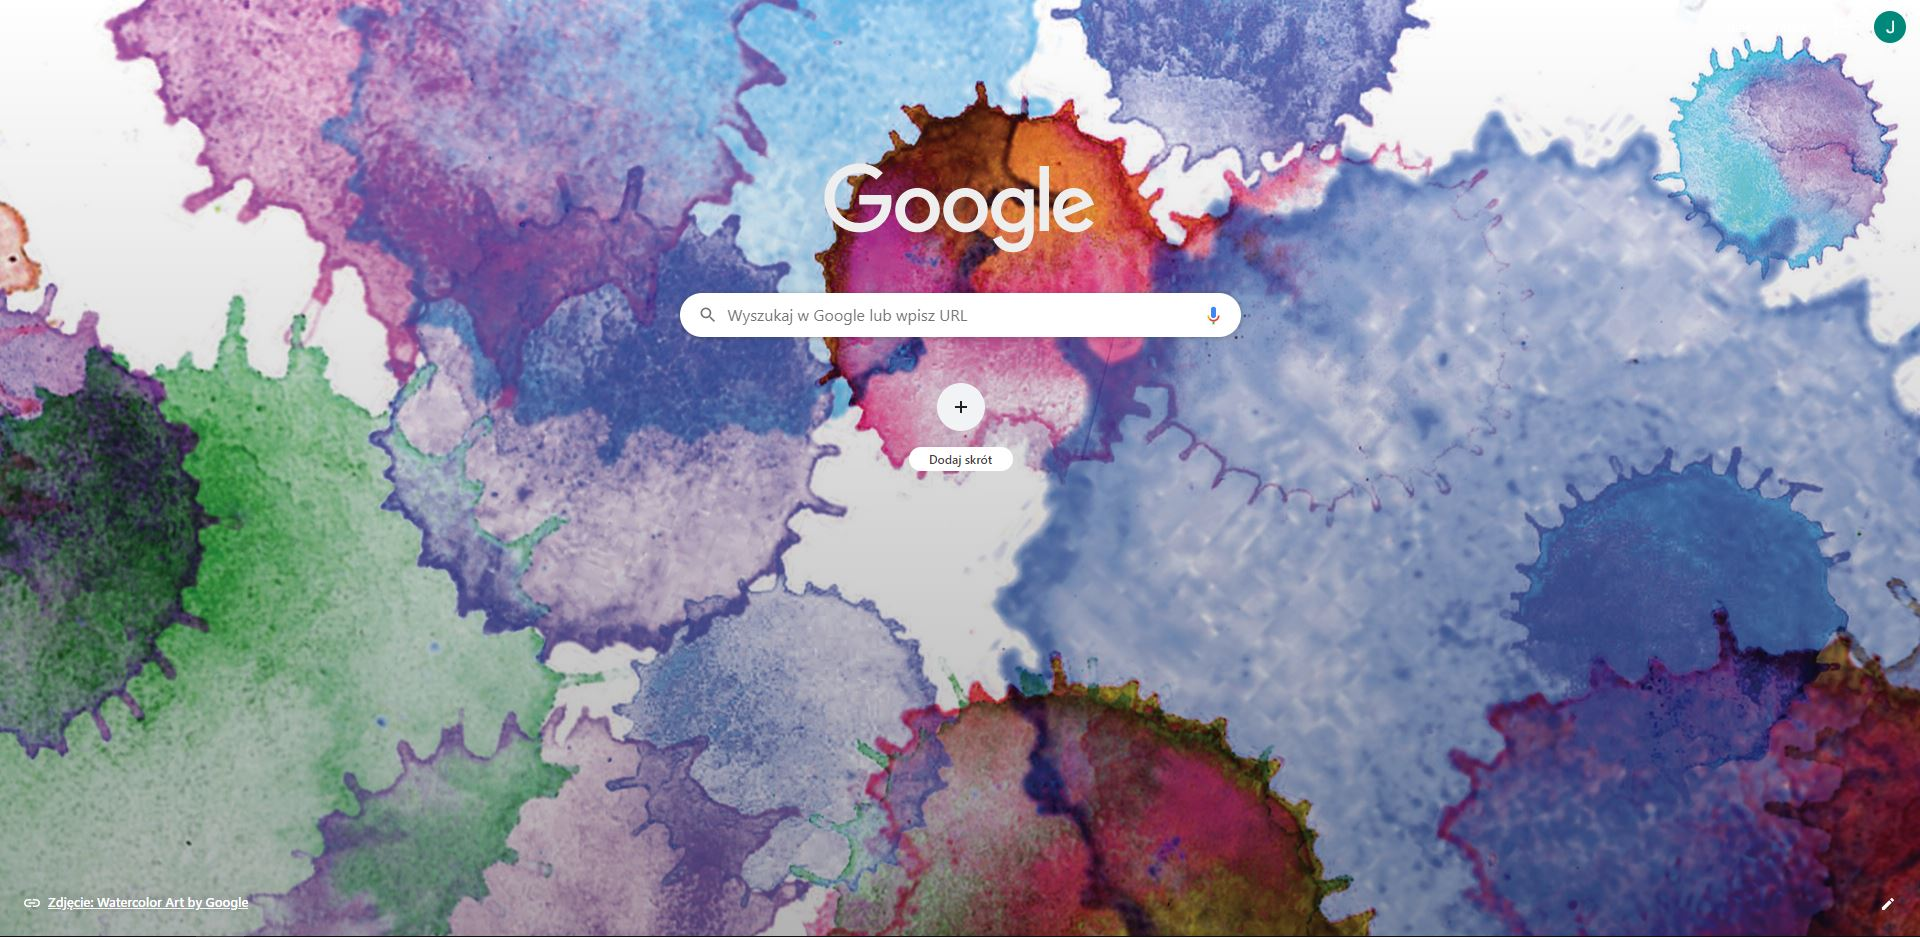
\includegraphics[width=\linewidth]{img/google-background}
	\caption{Główna strona wyszukiwarki Google ze skórką} \label{google-background}
	\endminipage\hfill 
	\minipage{0.49\textwidth}
	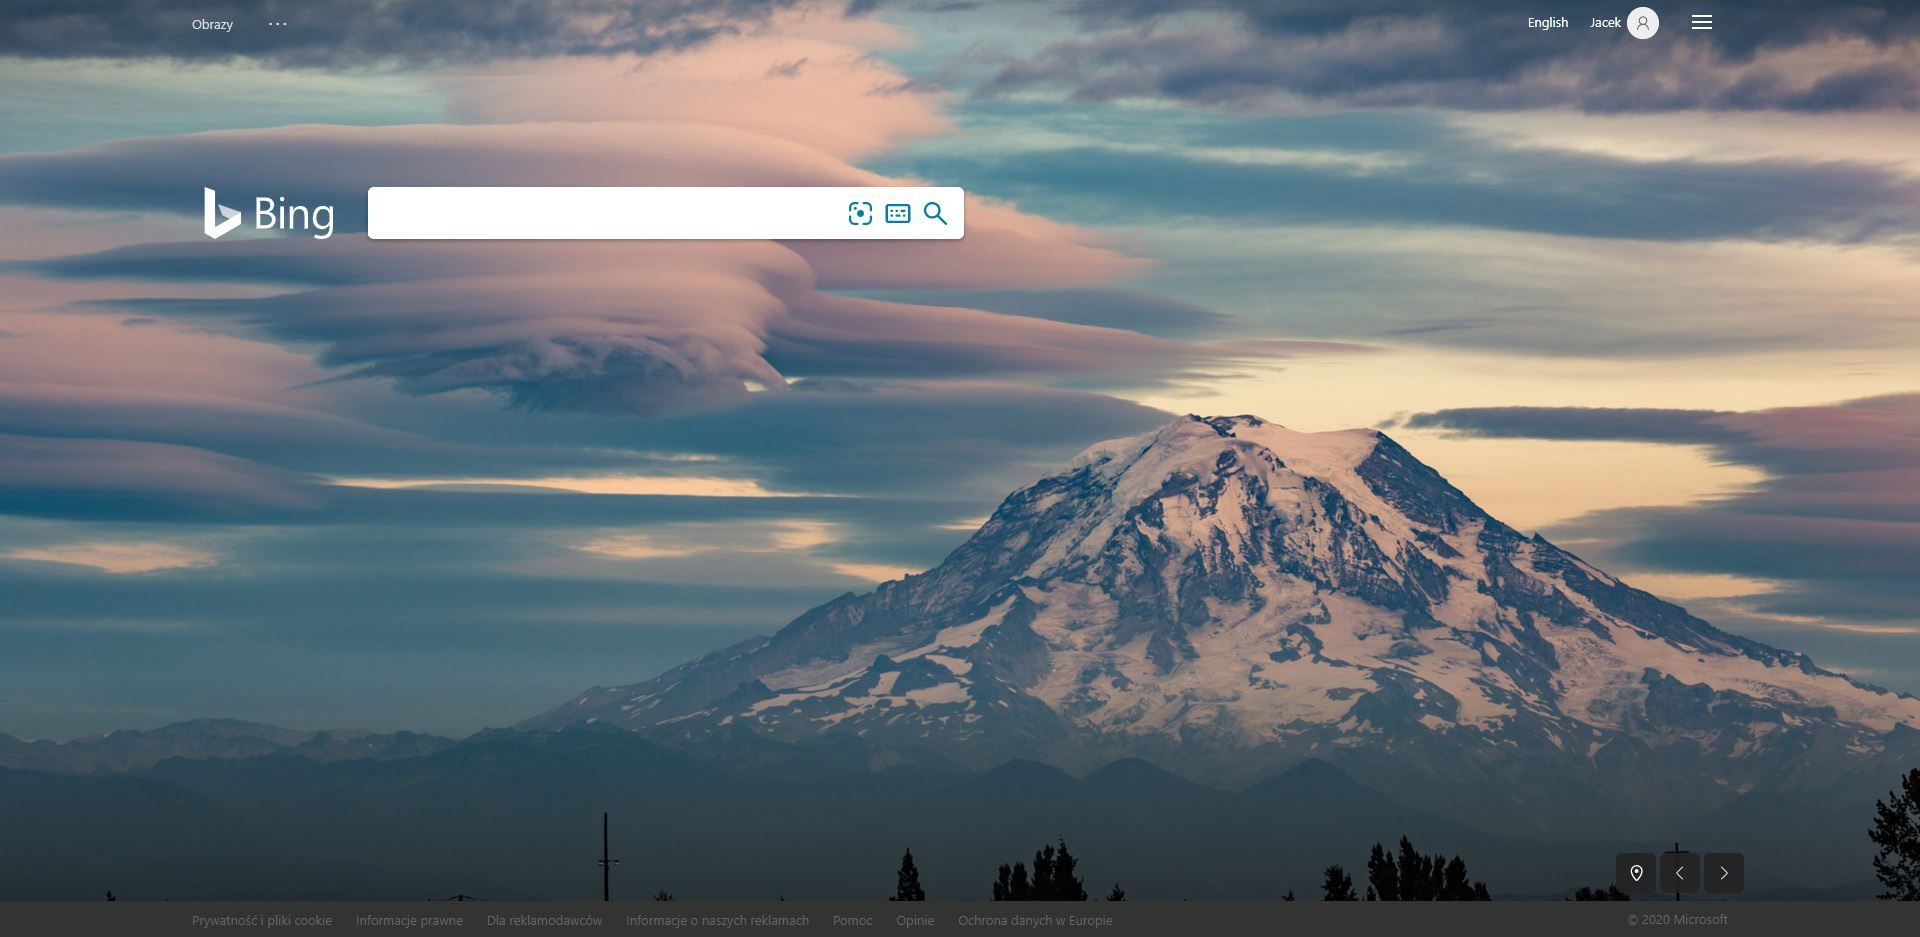
\includegraphics[width=\linewidth]{img/bing-background}
	\caption{Główna strona wyszukiwarki Bing ze skórką} \label{bing-background}
	\endminipage
\end{figure}

\section{Wyszukiwanie}

Po wpisaniu frazy, którą chcemy wyszukać obie wyszukiwarki wypiszą nam listę od kilkudziesięciu tysięcy do nawet kilkuset milionów rekomendowanych stron dla tego hasła.

Dla przykładu dla frazy ,,kobiety biznesu'' Google znalazło 125~000~000 wyników kiedy Bing zaledwie  341~000. Dominacja wyszukiwarki Google wśród użytkowników oraz zdecydowanie większa pula zaindeksowanych stron może być powodem dlaczego współcześni deweloperzy przygotowują swoje strony głównie pod pozycjonowanie wyszukiwarki Google.

\begin{figure}[!htb]
	\minipage{0.49\textwidth}
	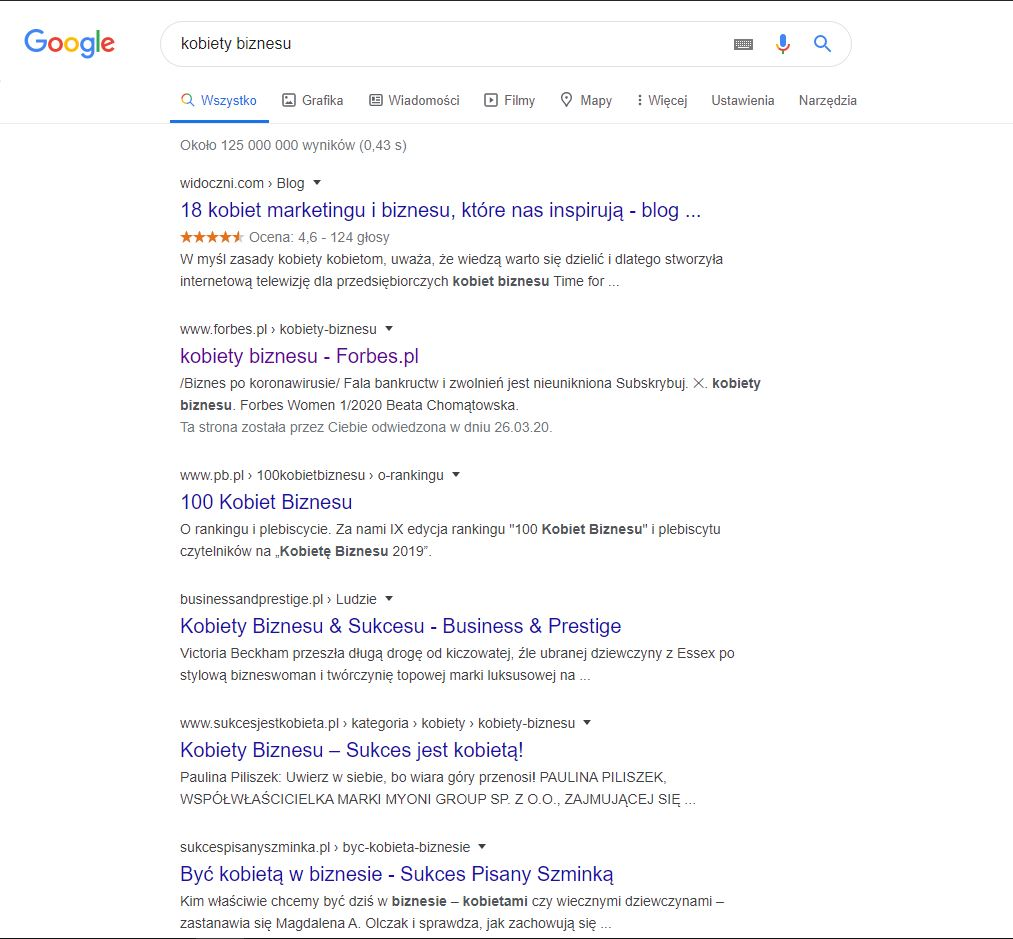
\includegraphics[width=\linewidth]{img/google-query}
	\caption{Lista rekomendowanych przez Google stron dla hasła: kobiety biznesu} \label{google-query}
	\endminipage\hfill 
	\minipage{0.49\textwidth}
	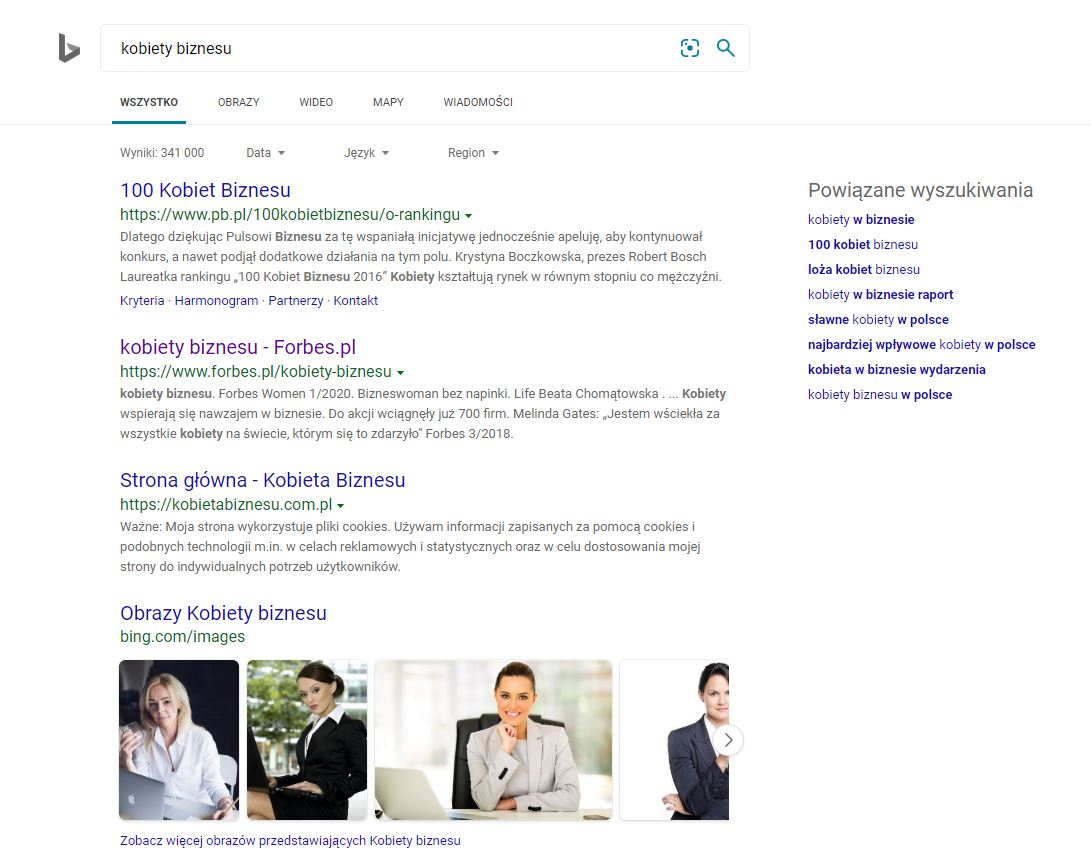
\includegraphics[width=\linewidth]{img/bing-query}
	\caption{Lista rekomendowanych przez Bing stron dla hasła: kobiety biznesu} \label{bing-query}
	\endminipage
\end{figure}


Każda z wyświetlanych pozycji przekazuje nam podstawowe informacje takie jak:
\begin{itemize}
	\item tytuł strony (zaznaczony kolorem zielonym)
	\item link do strony (zaznaczony kolorem fioletowym)
	\item skrót zawartości strony (zaznaczony kolorem brązowym)
\end{itemize}


\newpage

\begin{figure}[!htb]
	\minipage{0.49\textwidth}
	
\includegraphics[width=\linewidth]{img/google-responseBody}
	\caption{Wyświetlana pozycja w liście wyników google} \label{google-responseBody}
	\endminipage\hfill 
	\minipage{0.49\textwidth}
	
\includegraphics[width=\linewidth]{img/bing-responseBody}
	\caption{Wyświetlana pozycja w liście wyników bing} \label{bing-responseBody}
	\endminipage
\end{figure}

\begin{figure}[!htb]
	\minipage{0.49\textwidth}
	
\includegraphics[width=\linewidth]{img/google-responseBodyPlus}
	\caption{Wyświetlana pozycja w liście wyników Google z zaznaczonymi obszarami} \label{google-responseBodyPlus}
	\endminipage\hfill 
	\minipage{0.49\textwidth}
	
\includegraphics[width=\linewidth]{img/bing-responseBodyPlus}
	\caption{Wyświetlana pozycja w liście wyników Bing z zaznaczonymi obszarami} \label{bing-responseBodyPlus}
	\endminipage
\end{figure}

Oprócz podstawowego wyszukiwania linków do stron, mamy możliwość wybrania kategorii przedstawione na rysunkach~\ref{google-category} i \ref{bing-category} takich jak:
\begin{itemize}
	\item grafika
	\item wiadomości
	\item filmy
\end{itemize}

\begin{figure}[!htb]
	\minipage{0.49\textwidth}
	
\includegraphics[width=\linewidth]{img/google-category}
	\caption{Kategorie i filtry wyszukiwania Google} \label{google-category}
	\endminipage\hfill 
	\minipage{0.49\textwidth}
	
\includegraphics[width=\linewidth]{img/bing-category}
	\caption{Kategorie i filtry wyszukiwania Bing} \label{bing-category}
	\endminipage
\end{figure}

Ponadto wyszukiwarki dają nam możliwość intuicyjnego filtrowania wyników. W tym punkcie wyszukiwarki nieznacznie się różnią, gdyż Bing oferuje takie parametry jak: data, język, region. Natomiast Google: data, język i możliwość pokazania dokładnych wyników zawężając o wyniki fraz bliskoznacznych. 

\section{Podstawowe operatory}
Aby podnieść jakość i zawęzić pole poszukiwań pożądanych informacji przez użytkownika, Google zaimplementowało tak zwane operatory. 
Operatory definiują zakres poszukiwań poprzez słowa i znaki kluczowe:
\begin{itemize}
	\item \emph{" "} - wpisując wyrażenie w cudzysłów wymusza ścisłe dopasowanie. 
	Przykład: fraza \emph{"Steave Jobs"} wpisana z cudzysłowem wymusza aby w wyniku były dokładnie te dwa słowa obok siebie.
	
	\item \emph{OR} - operator logiczny pozwalający z zapytanie \emph{Steave OR Jobs} wyszukać wyniki zawierające frazę \emph{Steave} lub \emph{Jobs} lub oba.
	Operator można zastąpić znakiem $|$.
	
	\item \emph{AND} - domyślny operator logiczny, wyświetlający tylko te wyniki, które zawierają frazę \emph{Steave} i \emph{Jobs}. Operator jest domyślny więc przydatny jest tylko w połączeniu z innymi operatorami.
	
	\item $-$ - operator wykluczający. W przykładzie \emph{jaguar speed -car} wynikiem będą strony powiązane z frazą \emph{jaguar speed} ale niezawierające \emph{car}. Zatem chodziło nam o znalezienie prędkości jaguara będącego zwierzęciem a nie samochodem.
	
	\item \emph{..} - operator zakresu liczb. Przykład: \emph{podatki 2010..1015} da nam wynik wyszukiwania związanymi z podatkami miedzy 2010 a 2015 rokiem.
	
	\item \emph{( )} - operator grupowania fraz z innymi operatorami. 
	Przykład: \emph{(iPad OR iPhone)apple}. Operator \emph{AND} jest domyślny więc nie jest obowiązkowy.
	
	\item \emph{define:} - operator wyszukuje definicje szukanej frazy.
	
	\item \emph{filetype:} lub \emph{ext:} - operator określający rodzaj pliku będący wynikiem wyszukiwania takie, jak pdf, docx, txt, ppt.
	Przykład: \emph{Steve Jobs ext:pdf} - wyświetli tylko pliki pdf związane ze Steve'em Jobs'em. 
	
	\item \emph{site:} - ogranicza wyniki wyszukiwania tylko do jednej strony lub domeny.
	Przykład: \emph{wniosek site:.gov.pl} wyszuka informacje o wnioskach tylko na stronach rządowych kończących się na \emph{.gov.pl}.

	\item \emph{inurl:} - operator przeszukuje podaną frazę tylko w adresie url strony.
		
	\item \emph{intitle:} - operator przeszukuje podaną frazę tylko w tytule strony.
	
	\item \emph{intext:} - operator przeszukuje podaną frazę tylko w treści strony. Pominie strony zawierające frazę w tytule czy adresie url.
	
\end{itemize}

Google zawiera znacznie więcej operatorów. Niektóre z nich wymienione są na stronie sites.google.com \cite{operatory-google}

\chapter{Rekomendacja stron www}
\section{Algorytm}
Cały algorytm możemy podzielić na dwa etapy: indeksowanie i wyszukiwanie.
Użytkownik oczekuje od aplikacji szybkiego i trafnego wyszukiwania jednak, aby tak się stało trzeba najpierw zebrać wszystkie dane i nadać im specjalną strukturę dzięki której będziemy mogli szybko znaleźć interesującą nas informacje. To właśnie nazywamy procesem indeksowania.
\subsection{Proces indeksowania}
\subsection*{Document}
\subsection*{Analyzer}
\subsection*{Struktura indeksu}
\subsection{Proces wyszukiwania}
\section{Dodatkowe funkcje składni zapytania}

\chapter{Przedstawienie problemu i sposób jego rozwiązania}
\linia
\begin{itemize}
	\item Przede wszystkim przedstawienie tego problemu, który będzie opisany w pracy
	\item problem przedstawiony w pracy może być jednym z podproblemów ogólnego problemu biznesowego
	\item opis metod lub algorytmów np w postaci pseudokodu lub schematów 
	\item uzasadnienie użytych metod
	\item testy kilku parametrów, przygotowanie danych itd.
\end{itemize}

\linia

\chapter{Funkcjonalność zaimplementowanego systemu}
\linia
\begin{itemize}
	\item opis jakie funkcjonalności będzie miał system
	\item w jaki sposób dana funkcjonalność przyczyni się do rozwiązania problemu
\end{itemize}

\linia

\chapter{Implementacja oraz użyte technologie}
\linia
\begin{itemize}
	\item dokładnie jak zostało to wszystko implementowane
	\item opis architektury
	\item jaka platforma, diagram klas, jaka funkcjonalność jest w jakiej klasie/module/package
	\item opis głównych metod (nie opisujemy wszystkich metod)
	\item parametry jakie ma aplikacja, opis instalacji
\end{itemize}

\linia
\section{Java}
\subsection{Apache Lucene}
\section{Spring Boot}
\section{Thymeleaf}
\section{HTML}
\section{Struktura i działanie klas programu}
\subsection{Klasy silnika wyszukiwania}
\subsection{Klasy kontrolera}


\chapter{Przypadki użycia}
\linia
\begin{itemize}
	\item co dokładnie trzeba zrobić, aby zrealizować daną funkcjonalność
	\item zrzuty ekranu
\end{itemize}
\linia

\chapter{Podsumowanie}
\linia
\begin{itemize}
	\item ok 1-2 str
	\item cel pracy udało się osiągnąć
	\item w jaki sposób udało się osiągnąć cel z rozdziału 1 (w których rozdziałach jest to opisane)
	\item napotkane problemy
	\item w jaki sposób można aplikację/system udoskonalić
\end{itemize}

\linia
\cite{google-power-searching}

\bibliography{bibliografia} 
\bibliographystyle{ieeetr}
	
	


\end{document}